% % % % % % % % % % % % % % % % % % % % % % % % % % %
% % % % % % % % % % % % % % % % % % % % % % % % % % %
\section{BLE Schematic and PCB layout}
The Schematic of the Inventvm BLE modules is inherited directly from the vendors, which are BluEnergy-355MC\cite{BLNRG355_STEVAL_GUIDE} and Nordic nRF52840\cite{NORDIC_nrf52840_USERGUIDE}. The Figure\ref{fig:Nordic_ST_modules} shows the pinout and shape of the BLE module, which is multi-purpose because of same shape and pinout from both the BluEnergy-355MC and Nordic nRF52840 modules. By having the Same pinout and shape with different Bluetooth hardware, customers can use different Bluetooth hardware stacks with the same BMS solution. This approach is nothing but the daughter and motherboard approach where the Bluetooth module becomes the daughter board and BMS MMU board and CMU boards become motherboards.

\begin{figure}[h]
	\centering
	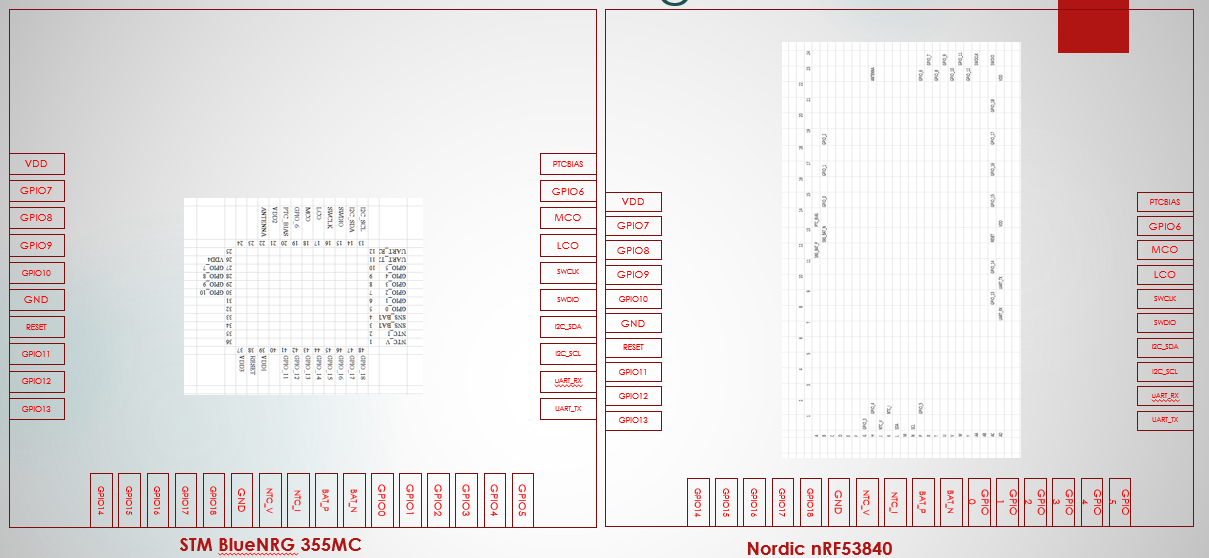
\includegraphics[width=0.7\textwidth]{Chap03/Figures/Nordic_ST_modules.PNG}
	\caption{BluEnergy-355MC(right) and Nordic Modules(left) }
	\label{fig:Nordic_ST_modules}
\end{figure}

\subsection{BluEnergy-355MC}
BLUENRG-355MC\cite{BLNRG355_STEVAL_GUIDE} BLE module includes BlueNRG-LP BLE low energy system on chip (QFN48 package), Associated with BlueNRG-LP development software stack from STM. The BlueNRG-LP features a 64 MHz, 32-bit Arm®Cortex®-M0+core, a 256 KB programmable flash memory, a 64 KB SRAM, an MPU, and an extensive peripheral set (6x PWM, 2x I²C, 2x SPI/I2S, SPI, USART, UART, PDM, and 12-bit ADC SAR)\cite{BLNRG355_STEVAL_GUIDE}. It is compliant with the Bluetooth® LE specification and supports master, slave, and simultaneous master-and-slave roles. It features data length extension, 2 Mbps, long-range, extended advertising and scanning, as well as periodic advertising, periodic advertising sync transfer, LE L2CAP connection-oriented channel, and LE power control and path loss monitoring\cite{BLNRG355_STEVAL_GUIDE}.
For more technical details refer STM BLUENRG-355MC datahseet \cite{BLNRG355_STEVAL_GUIDE}.
\subsubsection{BluEnergy-355MC RF Schematic:}
The Figure\ref{fig:STM_BLE_Schematic} refers to the core circuit of the BLUeNRG circuit for the Bluetooth, the pi network matching topology used to match the Ic and antennas, and refer \ref{fig:STM_BLE_Schematic} circuit between the RF net and the ANT net in the schematic.
All the discrete components are selected 0402 packages to make the Bluetooth module as sophisticated as possible, for more insight into the component selection for the schematic \ref{fig:STM_BLE_Schematic} refer to BOM\cite{BLNRG355_STEVAL_BOM}.
\begin{figure}[h]
	\centering
	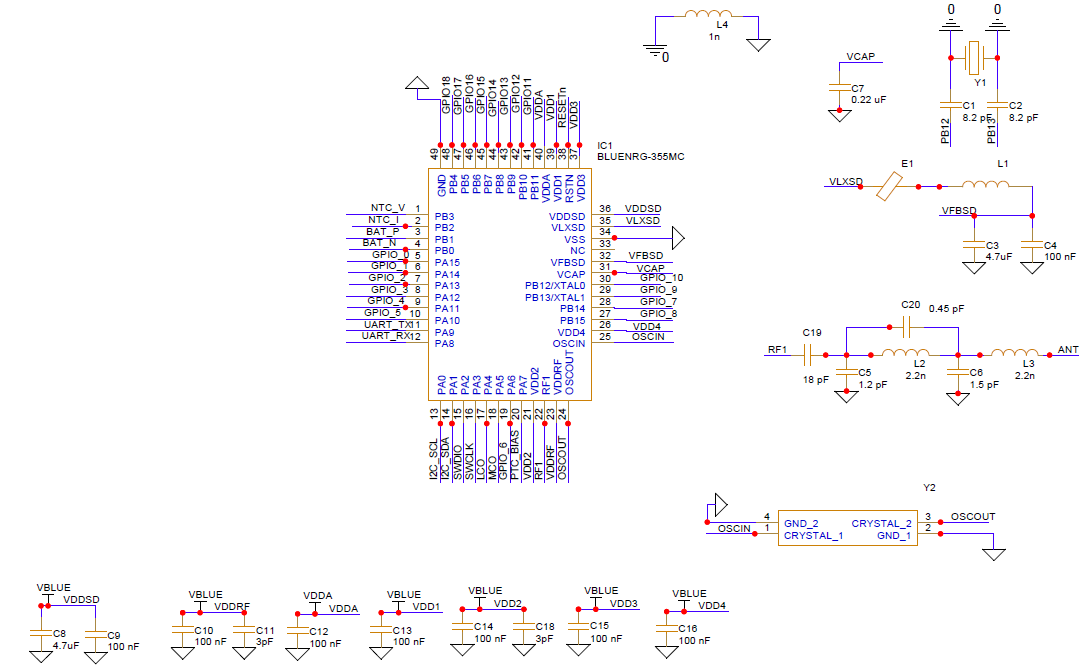
\includegraphics[width=0.7\textwidth]{Chap03/Figures/STM_BLE_Schematic.PNG}
	\caption{BluEnergy-355MC Module Core circuit }
	\label{fig:STM_BLE_Schematic}
\end{figure}

\subsubsection{BluEnergy-355MC RF Layout:}
The BLE module designed for the BMS application in Inventvm is the four-layer PCB, among four layers bottom layer is entirely dedicated to the ground. The bottom layer ground of the module is the analog ground it is differentiated from the power ground of the BMS from a small inductor to make sure the RF circuit gets less noise from the power ground. \\
\indent By referring to the layout Figure \ref{fig:BLE_PCB_ground_and_power_planes}of the RF module you can recognize that the shape of the power plane in the layer is pretty much weird, there is an RF technique behind making this kind of shape to avoid as much as the ground and power plane over a lap to decrease the capacitive parasitic effect. Parasitic components on PCB are the plague of the RF circuit, they can kill RF signal. Hence it is always a good idea to avoid power and ground planes overlap as much as possible and also make separate ground for the RF layout apart from the power ground.\\
\indent Place as many as vias possible from the top to bottom ground layer to enhance the ground layer capacity, and making sure to have equal space for antenna and RF feed line from the ground enhances the matching capability of the antenna. The following extinctions can give a detailed view of RF layout design:.

%%%%%%%%%%%%%%%%%%%%%%%%%%%%%%%%%%%%%%%%%%%%%%%%%%%%%%%%%%%%%%%%%%%%%%%%%%%%%%%%%%%%%%%%%%%%%%%%%%%%%%
%%%%% RF layout design guide lines 
%%%%%%%%%%%%%%%%%%%%%%%%%%%%%%%%%%%%%%%%%%%%%%%%%%%%%%%%%%%%%%%%%%%%%%%%%%%%%%%%%%%%%%%%%%%%%%%%%%%%%%

\begin{itemize}
	\item {\textbf{Power plane and Grounding :}}The power and Ground plane's overlap needs to be decreased as much as possible to avoid the parasitic capacitance effect. The Figure \ref{fig:BLE_PCB_ground_and_power_planes} refers to the power supply plane in the layer and the ground in the bottom layer.
		\begin{itemize}
			\noindent
			\begin{figure}[h]
				\centering
				\subfigure[Ground plane "Bottom layer"]{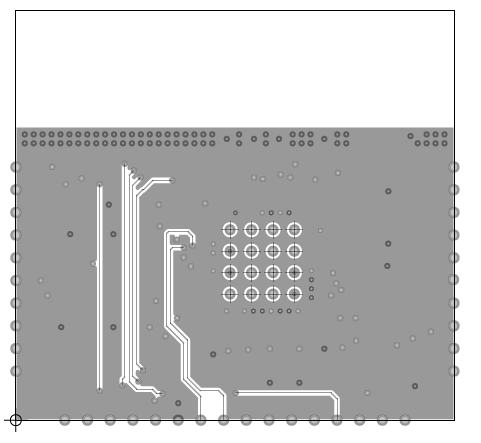
\includegraphics[scale=.6]{Chap03/Figures/nordic_module_grounding.PNG}}
				\qquad
				\subfigure[Power Plane "Layer 1"]{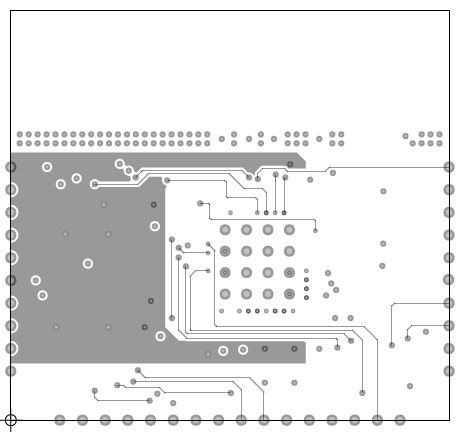
\includegraphics[scale=.6]{Chap03/Figures/Nordic_module_power_plane.PNG}}
				\caption{BLE PCB ground and power planes}
				\centering
				\label{fig:BLE_PCB_ground_and_power_planes}
			\end{figure}
		\end{itemize}
	\item \textbf{Equal Clearance to Antenna Feed :} It is essential to keep the same clearance throughout the RF feed line from the ground. This strategy helps to make equal parasitic capacitance from the ground. With an equal parasitic capacitance from the opposite side, the RF sanding wave reflections can be nullified. Figure\ref{fig:Antenna_Feed_clearence} depicts one such example of designing the RF feed line.
		\begin{itemize}
			\item \begin{figure}[h]
			    \centering
				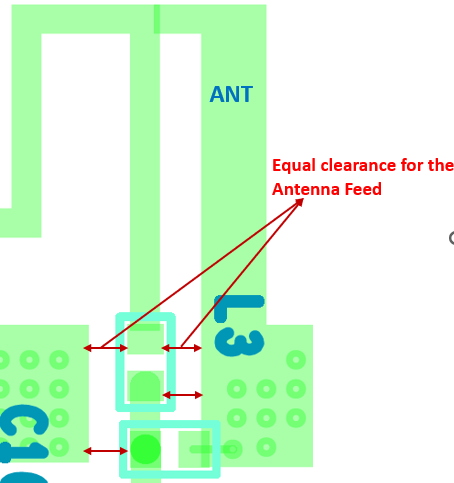
\includegraphics[width=0.4\textwidth]{Chap03/Figures/Antenna_Feed.PNG}
					\caption{Antenna Feed Line clearence}
					\label{fig:Antenna_Feed_clearence}
				\end{figure}
		\end{itemize}
	\item \textbf{ Isolate Power Ground from Analog/RF ground :}It is the most common practice while RF layout designing, The RF layout is isolated from the Power circuit. For this approach I have few intuitions behind the two-fold, those are :
		\begin{enumerate}\label{en:RFGND_isolation_benifits}
			\item RF-related noise is confined within the RF/Analog ground of the PCB.
			\item This will isolate noise from the digital circuitry with the DC power supply and High power switching circuit on the BMS board.
			\item RF circuit protected from direct current flow from DC supply if there are any power surges in supply. So on....
		\end{enumerate}
	    \begin{figure}[h]
			\centering
			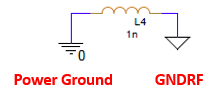
\includegraphics[width=0.4\textwidth]{Chap03/Figures/PGND_GNDRF_Isolation.PNG}
				\caption{Power Ground and RF Ground Isolated with Inductor}
				\label{fig:PGND_GNDRF_Isolation}
		\end{figure}
		\ref{en:RFGND_isolation_benifits} Such mentioned benefits can be obtained by placing an inductor between the Power Ground/RF ground. Choosing Inductor for such functionality follows that the inductor will not allow sudden current spikes $L\times \frac{d i}{d t}$ , on the benefit it can also provide a high current ratio when the current is stable,reference \ref{fig:PGND_GNDRF_Isolation}..
	\item \textbf{ RF feed line shape :}It is common practice to keep the rf feed line with the known shape. Since Bluetooth operates at 2.4GHz, even one millimeter can give a large amount of resonant frequency drift in antenna reflections. The simplest approach to mitigate such issues is to keep the RF feed and the RF IC, both on the same axis. To avoid unnecessary parasitics by an irregular shape of the antenna, make a feed trace from the ic to Antenna with the same width as the antenna feed has. Figure \ref{fig:Antenna_Feed_Shape} shows the approach that I have followed to design the Antenna feed and the RF trace, The Figure shows the nonregular shape of the antenna.
			\begin{itemize}
				\item 
				\begin{figure}[h]
					\centering
					\subfigure[Regular shape and Antenna feed]{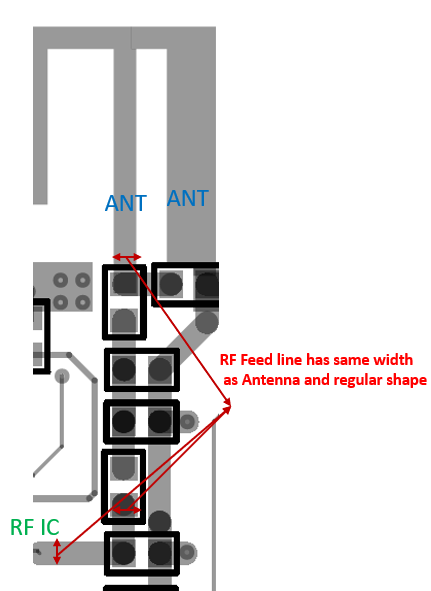
\includegraphics[scale=.6]{Chap03/Figures/Regular_Antenna_feed.PNG}}
					\qquad
					\subfigure[Irregular Antenna shape and Antenna feed]{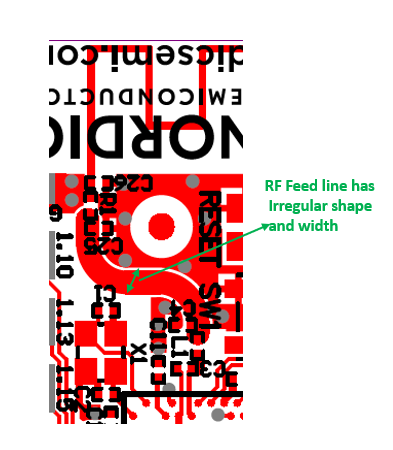
\includegraphics[scale=.6]{Chap03/Figures/Irregular_antenna_feed.PNG}}
					\caption{Antenna Feed Shape}
					\centering
					\label{fig:Antenna_Feed_Shape}
				\end{figure}
			\end{itemize}
	\item \textbf{Grounding Via's :} Keep always clean ground and this can be achieved by placing as many vias from the top layer to the dedicated RF/Analog ground in the bottom layer. It is recommended in the PCB design to place the Vias with equal distance, Figure \ref{fig:Antenna_Feed_Shape} refers to Vias placement from the top layer to the bottom layer with equal distance. There should not be any ground under the RF antenna, because the ground under the RF antenna again makes, Antenna just an RF trace instead of allowing open radiation.
	\begin{itemize}
		\item 
		\begin{figure}[h]
			\centering
			\subfigure[Top Layer Vias]{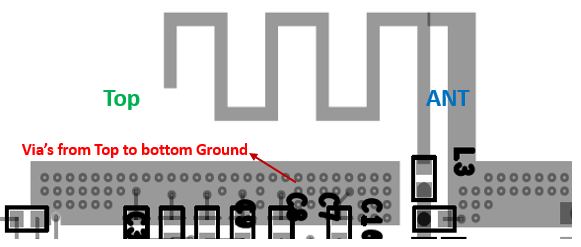
\includegraphics[scale=.5]{Chap03/Figures/Top_vias.PNG}}
			\qquad
			\subfigure[Bottom Layer Vias]{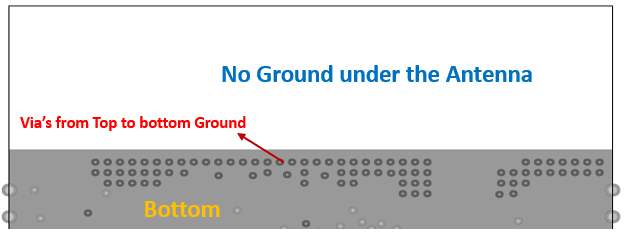
\includegraphics[scale=.5]{Chap03/Figures/Bottom_vias.PNG}}
			\caption{Vias placement on BLE board}
			\centering
			\label{fig:BLE_Module_Vias_Placement}
		\end{figure}
	\end{itemize} 
	\item \textbf{Antenna placement :} Do not place any component in the Antenna Keep out area, make the strict keep-out area for the antenna to prevent any external components' noise interference. It is always good placement to avoid any of the plastic components around the antenna because the plastic can behave like a dielectric and this will change the antenna characteristics. Antenna placement on they should end of the PCB where the PCB notch is pointed out. See Figure\ref{fig:BLE_PCB_ground_and_power_planes} the antenna has been placed on the edge of the PCB and there are no plastic or high-frequency switching circuits around it.
\end{itemize}

\subsubsection{Power Supply Decoupling Layout Considerations\cite{AN91445}}
Note the following best practices when laying out the power supply traces:
\begin{itemize}
	\item Place the components as close to the supply pin as possible \cite{AN91445}.
	\item Place the smallest-value capacitor closest to the power supply pin \cite{AN91445}.
	\item Place the decoupling capacitor on the same layer as the IC. If it is not possible to place all the capacitors on the same layer, give priority to smaller values \cite{AN91445}.
	\item The power supply should flow through the decoupling capacitors to the power supply pin of the IC. Avoid using
	\item supply vias between the component and the pin \cite{AN91445}.
	\item Use separate vias to ground for each decoupling capacitor. Do not share vias\cite{AN91445}.
	\item For four-layer boards with a separate power plane, use separate vias for each power supply pin to the power plane \cite{AN91445}.
	\item It is recommended not to share the vias \cite{AN91445}.
	\item Some of the commonly made layout issues related to power supply decoupling are shown in \cite{AN91445} Figure \ref{fig:Power_Supply_Decoupling}.
\end{itemize}
\begin{figure}[h]
	\centering
	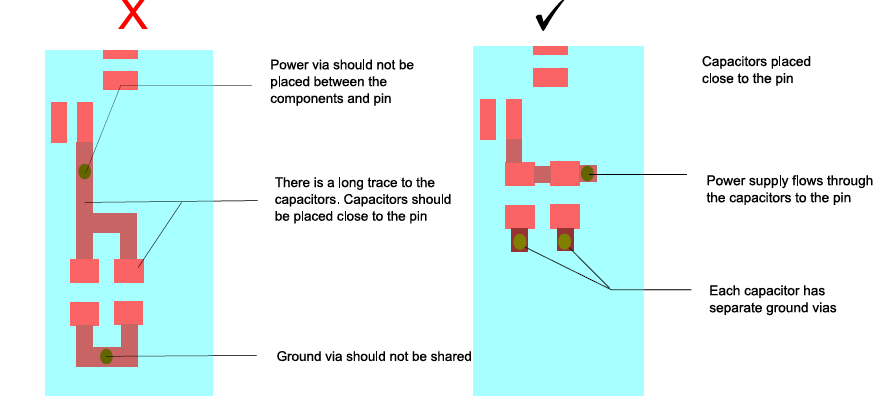
\includegraphics[width=0.7\textwidth]{Chap03/Figures/power_supply_coupling.PNG}
		\caption{Power Supply Decoupling}
		\label{fig:Power_Supply_Decoupling}
\end{figure}

%%%%%%%%%%%%%%%%%%%%%%%%%%%%%%%%%%%%%%%%%%%%%%%%%%%%%%%%%%%%%%%%%%%%%%%%%%%%%%%%%%%%%%%%%%%%%%%%%%%%%%

\subsubsection{BluEnergy-355MC RF Matching Circuit Layout:}
It is always a good approach to have the matching circuit as tight as possible you can refer to the Figure\ref{fig:Antenna_matching_network} the matching circuit is placed as close as possible, to avoid any additional track length to create some extra RF stub effects.  Don't ever run any of the signal lines across the RF feed line and always make sure to place the IC and RF in the same direction this approach will avoid any strange track shapes which can cause parasitics. It is a good way to make sure the RF feed line to the antenna through the IC has the same width across the track length this will avoid any unnecessary filtering effect. The figure refers to all of above-mentioned RF layout design hints.
Figure\ref{fig:Antenna_matching_network} shows that matching components are tightly packed, and no signals run across the RF feed.

\begin{figure}[h]
	\centering
	\subfigure[Matching Network Layout]{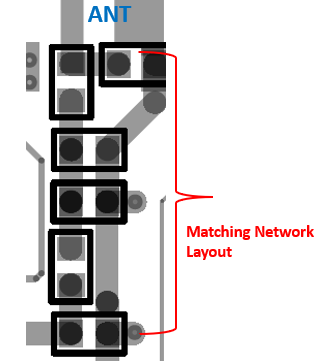
\includegraphics[scale=.8]{Chap03/Figures/matching_network_layout.PNG}}
	\qquad
	\subfigure[Matching Network Schematic]{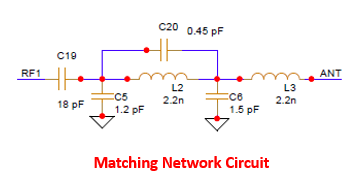
\includegraphics[scale=.8]{Chap03/Figures/matching_network_circuit.PNG}}
	\caption{BLE Antenna Matching Network}
	\centering
	\label{fig:Antenna_matching_network}
\end{figure}
We can place the components even overruling the component outline. Until we do not make the pads overlap, to achieve this we might have to bypass some PCB DRCs.

\subsection{Summary of the RF layout Design guidelines :}
\begin{enumerate}
	\item Keep Ground clearance as much as possible around the antenna.
	\item Make equi clearance on both sides of the antenna and RF feed line.
	\item Do not make a strange shape of the antenna feed line.
	\item Do not run any of the signal lines under the antenna or RF feed line.
	\item Make more vias from the top layer to the bottom layer for pure ground.
	\item Keep capacitive filters as near as possible to the power supply pins.
	\item Pack antenna matching network as close to antenna and IC RF feed.
	\item Place antennae in less clumsy are from other circuitry on the PCB.
	\item Make less overlap of the ground plane and power plane.
	\item Avoid high-frequency circuits around the RF feed.
	\item Always places the antenna at the edge of the PCB.
	\item Always chooses a standard pattern for the ground around the antenna.
	\item Never places any components, screws, mounting holes, or planes in the keep-out area of the antenna.
	\item The antenna must house with a Metalic shield to avoid external interference.
	\item There should not be direct ground under the antenna.
	\item The Orientation of the antenna should be inlined with the final PCB.
	\item When using the passive matching circuit try to have multiple components matching this can help at the debugging stage to tune the matching circuit.
\end{enumerate}

